\chapter{Terms and Explanations}
\label{appendix:termsexp}

\index{actors}
\section{Actors}

\index{user}
\index{end-user}
\subsection{End-user}
An end-user in the context of cion is a developer, usually with a degree in IT, and preferably in development or systems engineering.

The user deploys new images to dockerhub and/or docker registry.

\index{administrator}
\subsection{Administrator}
An end-user in the context of cion is a developer or operations manager, and usually with a degree in IT, preferably in operations or development.

The administrators use the cion web interface to configure cion's environments. 

\index{owner}
\subsection{Owner}
An owner is the entity that owns the servers and services that cion is to manage. These environments may or may not be where cion itself is running.

\index{developer}
\index{cion developer}
\subsection{Developers}
If not specified otherwise, these are the developers, designers and managers of cion as a product. They are not inherently the developers, owners or managers of the servers, environments or services that cion is running in or managing.

\index{environment}
\section{Environment}
An environment is where the docker services are running. Usually a company will have multiple environments with different permissions and integrations to external systems and requirements for uptime and security.

\subsection{Trondheim Municipality's environments}
These are the three different environments that the Municipality use.
\subsubsection{Production}~
This is where the services that serve the users run.

\index{prod}
\index{production}
\subsubsection{Production}


\index{QA}
\index{quality assurance}
\subsubsection{Quality Assurance}
This environment should be as close to the production environment as possible when it comes to specifications of the hardware. It is used to assure that software that is in development runs as it should, before deploying to production.

\index{testing}
\subsubsection{Testing}
This environment is used as a playground to test services while they are still in development.

\index{docker}
\section{Docker}
Docker is a container orchestration platform, allowing developers to isolate and manage running services.

\index{image}
\index{docker image}
\subsection{Docker image}
A docker image is an archive of files and instructions to instantiate an instance of an application/service.
\newline
An image has a name and a tag. Where the tag describes what version of the application the image contains. \newline
It has the following format: 

username/repository:versiontag

\index{hosting}
\subsection{Image hosting}

\index{registry}
\index{docker registry}
\subsubsection{Docker registry}
A registry is a server-side application that stores and serves docker images.

\index{dockerhub}
\index{repository}
\subsubsection{DockerHub}
DockerHub is a publicly hosted free service provided by Docker that acts as a Docker registry. These are referred to as repositories.

\index{push}
\index{pushing}
\index{image push}
\subsubsection{Pushing}

When a new version of an image is ready it can be pushed to a image host to make it available to everyone with access to that repository.

\index{pull}
\index{pulling}
\index{image pull}
\subsubsection{Pulling}

An image can be pulled from an image host to the local machine.

\index{container}
\index{docker container}
\subsection{Docker container}
A docker container is a running instance of an application and the sandbox the application is running in. It can be seen as a virtual machine, with its own file-system and user-system, where the only running process is the application itself.

\index{docker service}
\index{service}
\subsection{Docker service}
A service is an abstraction over containers. It consists of multiple running instances of the same image. The service-functionality in docker is only available when docker is running in swarm-mode. Docker will make sure that, through health checks in the containers, a certain amount of containers are running with the specified image.

\index{docker socket}
\index{socket}
\subsection{Docker socket}
Docker exposes a local management API over a unix socket located at \textbf{/var/run/docker.sock}.

\index{container orchestration}
\section{Container orchestration}
Container orchestration refers to the automation of managing containers. This process includes deploying new containers, updates to existing containers, scaling \index{scaling}(running multiple containers for the same service), removal, and inter-container communication.

\index{management api}
\index{api}
\section{Management API}
A management API refers to an API exposed by a service, that lets its requesters to change the configuration of the service through web-requests, for example over HTTP. It is then vulnerable by nature. In the example of docker, access to the management API could give the requester root access to the host-machine.

\index{swarm}
\index{swarm-mode}
\index{docker swarm}
\subsection{Docker Swarm}
Docker Swarm is Docker's answer to container orchestration. It allows the user to connect multiple docker environments across multiple hosts. A docker instance is referred to as \textit{running in swarm mode} when it is part of a Docker Swarm. Inside a Docker Swarm environment hosts are either \textit{workers} or \textit{managers}. And even though a Swarm can have multiple managers there is only \textbf{one} active manager at any given time, this host is referred to as the \textit{leader}. The leader is the only host that can manage the swarm, as in deploy new, update and remove services \& containers. 

\index{kubernetes}
\subsection{Kubernetes}
Kubernetes is an container orchestration system like Docker Swarm created by google. It allows IT professionals to abstract away multiple servers. Like Docker Swarm Kubernetes can depoy, update and manage running instances of docker images.

\index{programming concepts}
\section{Programming concepts}

\index{callback functions}
\subsection{Callback functions}
Callback functions are a functional programming concept where blocks of code are captured in variables, the callback function can be called like any other functions. 


\index{TLS termination proxy}
\index{TLS termination}
\section{TLS termination proxy}
A TLS termination proxy is a proxy that handles and decrypts TLS-encrypted requests and passes on the unencrypted request to the proxy's target and encrypts the unencrypted response from the target before sending it to the original requester.

\index{CI}
\index{CD}
\index{continuous integration}
\index{continuous delivery}
\index{continuous deployment}
\section{CI/CD}
CI/CD refers to continuous integration, continuous deployment and continuous delivery.

All of these concepts describe different levels of automation in the development cycle.


\begin{figure}[h!]
  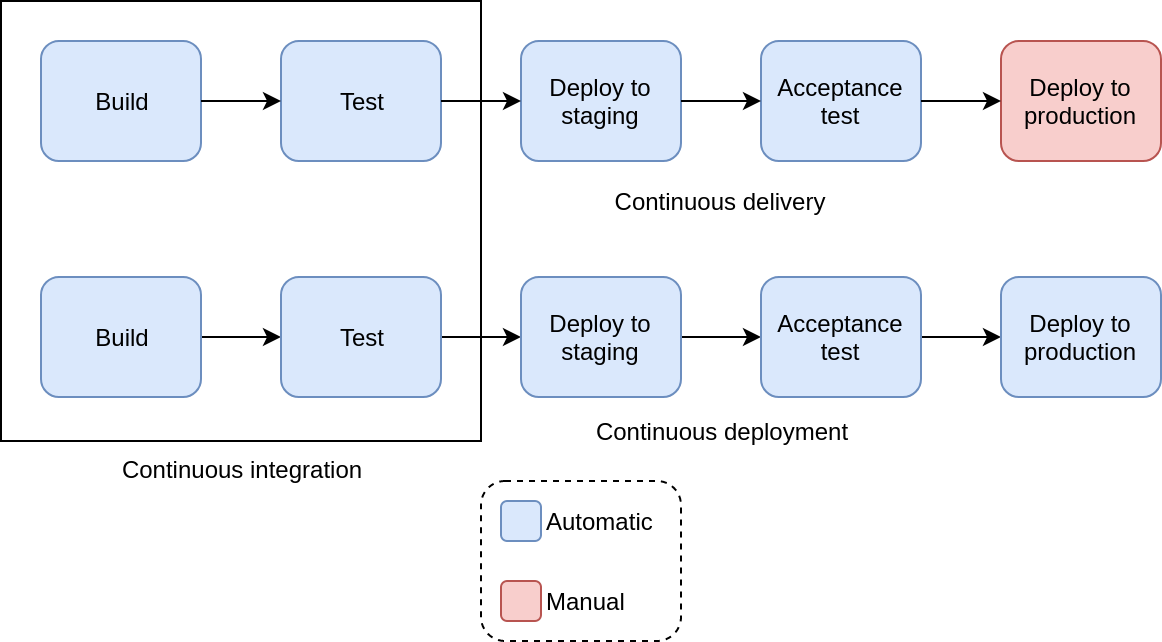
\includegraphics[width=\textwidth,height=\textheight,keepaspectratio]{images/ci_cd_comparison.png}
  \caption{CI/CD comparison}
\label{fig:CI/CD-comparison}
\end{figure}

Continuous integration is automation of building and unit-testing code. Continuous delivery extends this process and further automates deployment to staging-environments and running of acceptance tests or similar. Continuous deployment further extends it by automating deployment to production environments.

\index{webhook}
\section{Webhook}
A webhook is an HTTP POST-request that is triggered on some event to a receiver.
In the context of cion, a webhook is an HTTP POST request that is triggered when a new docker image has been uploaded to a docker image repository or registry. The webhook receiver is a running instance of the cion catalyst.

\index{healthcheck}
\section{Healthcheck}
A healthcheck is a periodic check that probes some aspect of an application to verify that it is running correctly. For a web-application a natural healthcheck is to run the \textit{curl}-command to simply check if one of its endpoints respond to a web-request.

\index{repository}
\index{code repository}
\section{Code Repositories}

\index{github}
\subsection{Github}
GitHub is a code repository where developers can upload their open-source projects.

\index{bitbucket}
\subsection{Bitbucket}
Bitbucket is a git-server with additional features by Atlassian. It can be self-hosted or accessed as a cloud service hosted by Atlassian.
\newline
The features beyond being a git-server include:
\begin{itemize}
    \item integration with the rest of Atlassian’s software, like:
    \begin{itemize}
        \item JIRA
        \item Confluence
    \end{itemize}
    \item Bitbucket pipelines, a CI/CD environment
    \item A web UI
\end{itemize}

\index{pipelines}
\subsubsection{Bitbucket pipelines}
Bitbucket pipelines is a CI/CD environment integrated with the Bitbucket git-server. It lets the user create scripts that run on specific triggers, like a git push to a specific branch of a repository.

\index{cion}
\index{cion solution}
\section{cion solution}


\index{cion task}
\index{task}
\subsection{Task}
A task refers to an action that is not yet performed, and is stored in the database waiting to be picked up by the cion orchestrator and then performed by a cion worker. A task can be pretty much anything that can be run as python code, but most tasks in the cion context are updates of services, or \textit{deployments}.

\index{task state}
\index{state}
A task can have one of multiple states. The default state is \textit{ready}.
The different states are:
\begin{itemize}
    \item\index{ready} ready: these tasks are not yet picked up by any cion component
    \item\index{processing} processing: this state indicates that a task is currently being handled
    \item\index{processed} processed: this state indicates that a task was completed successfully
    \item\index{erroneous} erroneous: this state indicates that a task was attempted but did not complete successfully
\end{itemize}

A task consists of multiple fields:
\begin{itemize}
    \item\index{task time} time: when the task was last updated. The initial value is when the task was created
    \item\index{task event} event: this field specifies what kind of task this is. And depending on this value different fields can be present
    \item\index{task data} Any data specific to the event kind
\end{itemize}

\index{cion interface}
\index{cion web}
\index{web}
\subsection{Web interface}
The cion web interface is a web-site that lets its users manage an instance of cion through a graphical user interface (GUI). Some of its features are:
\begin{itemize}
    \item user authentication and user management for the web GUI
    \item adding new environments for cion to manage
    \item adding and removing new services for cion to manage
    \item update services running in environments managed by cion
\end{itemize}

\index{deploy}
\index{deployment}
\subsubsection{Deployment}
A deployment refers to an update of a service. 


\index{api}
\index{cion api}
\index{application programmer interface}
\subsection{API}
The cion API is the backend of the web interface. It receives requests from users of the web-interface and authenticates users before making queries to the database.


\index{catalyst}
\index{cion catalyst}
\subsection{Catalyst}
The cion catalyst is the component of the cion solution that receives requests from for example webhooks from github or bitbucket pipelines. The catalyst reads these requests and publish tasks in the database. 

\index{cion backend}
\index{backend}
\subsection{Backend}
The cion backend is the component of the cion solution that gets tasks from the database and performs them. These \textit{tasks} can be for example a \textit{service-update} task, which refers to the deployment of a new update to the image of a running service.

\index{cion instance}
\subsection{Instance}
A cion instance refers to a running instance of cion. Deployed in a company's running service-environment. It has no inherent connection to cion's developers, and is managed by that company.

\newpage
\printindex